\documentclass[aip,amsmath, reprint, author-year]{revtex4-1}
\usepackage{url}
\usepackage[utf8]{inputenc}
\usepackage{hyperref}
\usepackage{graphicx} % for graphics
%\usepackage{listings} % for code listtings
%\usepackage{color}

%\setcitestyle{round, author-year}

\setcounter{page}{1}

%\bibliographystyle{aipauth4-1.bst}

\begin{document}

\begin{abstract}
A approach to generate Generalized Process Capability Data in order to populate and add functionality to a Process Capability Database.
A description of the concept of generalization, uses and implementation.
\end{abstract}

\title{Concept of using General Process Capability Data}
\author{Andreas Bruun Okholm, s082562\\
Mathias Rask Møller, s082536 }
\affiliation{Technical University of Denmark}
 
\date{\today}
\maketitle

%Introduction

\section{Introduction}

A Process Capability DataBase (PCDB)  is a tool for mechanical designers to get information of what is possible to achieve in the companys production. By applying PC information in the design process it is possible to reduces: rework, cost, failure rate, assembly problems and increases product performance.
A in few words a PCDB is a database of variance in features on produced products. Different companies have different index system and standards for what to record. 

As mentioned in (\cite{raskokholm} , unpublished) and (\cite{kern2003forecasting}) a number for key challenges has to be addressed to expand the use of PCDB.
\begin{itemize}
	\item Retrievable data: The database has to be populated with the desired data in a understandable manner.
	\item User Interface: Accessing the information should be easy.
	\item Organizational: Development department are dependent on data from production. 
	\item Information Technology: Make a database which is fast, live, global, self populating, up to date and live up to the industry criteria of security and anonymity.
\end{itemize}

\section{The right data}
For designer to use a PCDB in the design process, the database has to contain the needed data. The designers themselves does not generate the necessary data and from (Tata) we have learned that the data already recorded in the process control is not necessary the desired data for the mechanical designer. 

The data desired by the designer can be syntetisized to PC data of a geometry, material and process in order to design for what is achievable in production. 
The data recoded by process control can be processed to describe geometries for the process and material instead of specific features on a specific product thus making the process control data from one product, whose only similarity with the designed product is the geometrical features only, available for use for the designer.

\section{User Interface}
Availability of the data is important. The reward for using PCDB or robust design in general to make changes in early design is a long reach compared the reward for the hero in production solving the expensive errors in design. The importance of the tool being easy to use 

In order to make the mechanical designers use the tool, it is important that the data is easy to sort through and make decisions of what is the desired information, and then find it.

\section{Predicting Process Capability}
The process capability indices ($C_p$ and $C_{pk}$) described by \cite{kane1986process} has been widely adopted in statistical process control, been extended and further researched for better understanding \citep{wu2009overview}. 
Instead of looking at process mean $\mu$, standard deviation $\sigma$ and specification upper and lower limits $USL$, $LSL$ using Process Capabilities Indices (PCIs) transforms these values into unit less numbers, which provides a quick overview of how a process is performing.

The PCIs ability to transform process variables of any object into unit less capability index can be reversed to calculate desirable specification limits. For en example the commonly used CPI $C_pk$ 
\begin{equation}
	C_{pk} = \frac{d - | \mu - m|}{3 \sigma}
\end{equation}
can be reversed
\begin{equation}
	d = 3 C_{pk} \sigma + | \mu - m|
\end{equation}
where $d = (USL - LSL) / 2$ is half the specification limit and $m = (USL + LSL) / 2$ is the midpoint between the specification limits. 

The most common PCIs and what they describe \citep{wu2009overview, taguchi1986introduction}
\begin{itemize}
	\item $C_a$ : Closeness of process mean to target 
	\item $C_p$ : Relative size of variation
	\item $C_{pk}$ : Amount of nonconforming (\%NC)
	\item $C_{pm}$ : Value loss (Taguchi loss function)
	\item $C_{pmk}$: Version of $C_{pm}$,  sensitive to mean shift. 
\end{itemize}

For the purpose of our database we have chosen to use $C_{pk}$, since it provides the most easily understandable result. The desired specification limit will result in a maximum percentage of NC products. Using $C_{pm}$ would be sensible sense if the desired tolerances directly influence product performance - for instance in optics construction.  




\cite{tang1997graphical}


ISO 286? describes a non-linear function for comparing tolerances on objects of different dimension. This function used to normalize tolerances and display PC independent of size (with in the limits of the function.)  

confidence intevals

\section{How much data}


\begin{figure}
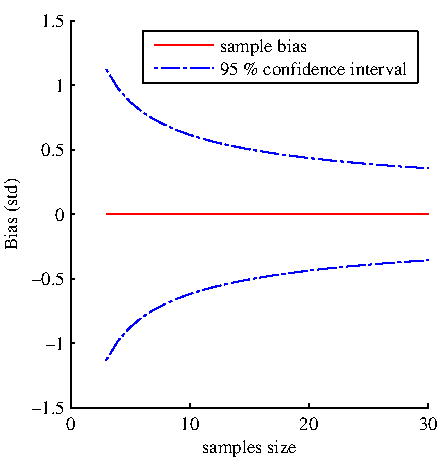
\includegraphics{stats_bias_confidence.pdf}
\caption{\label{fig:std_uncertainty}The uncertainty of the standard deviation estimate is reduced as the number of samples is increased. The increase in accuracy gained per additional decreases with more samples. From the graph we have chosen 12 to be the optimal point for general process capability use.}
\end{figure}



\begin{figure}
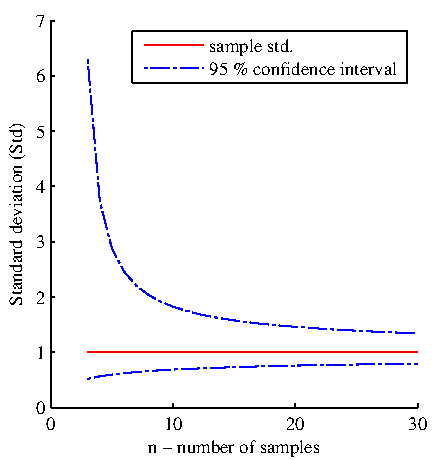
\includegraphics{stats_std_confidence.pdf}
\caption{\label{fig:std_uncertainty}The uncertainty of the standard deviation estimate is reduced as the number of samples is increased. The increase in accuracy gained per additional decreases with more samples. From the graph we have chosen 12 to be the optimal point for general process capability use.}
\end{figure}


\begin{figure}
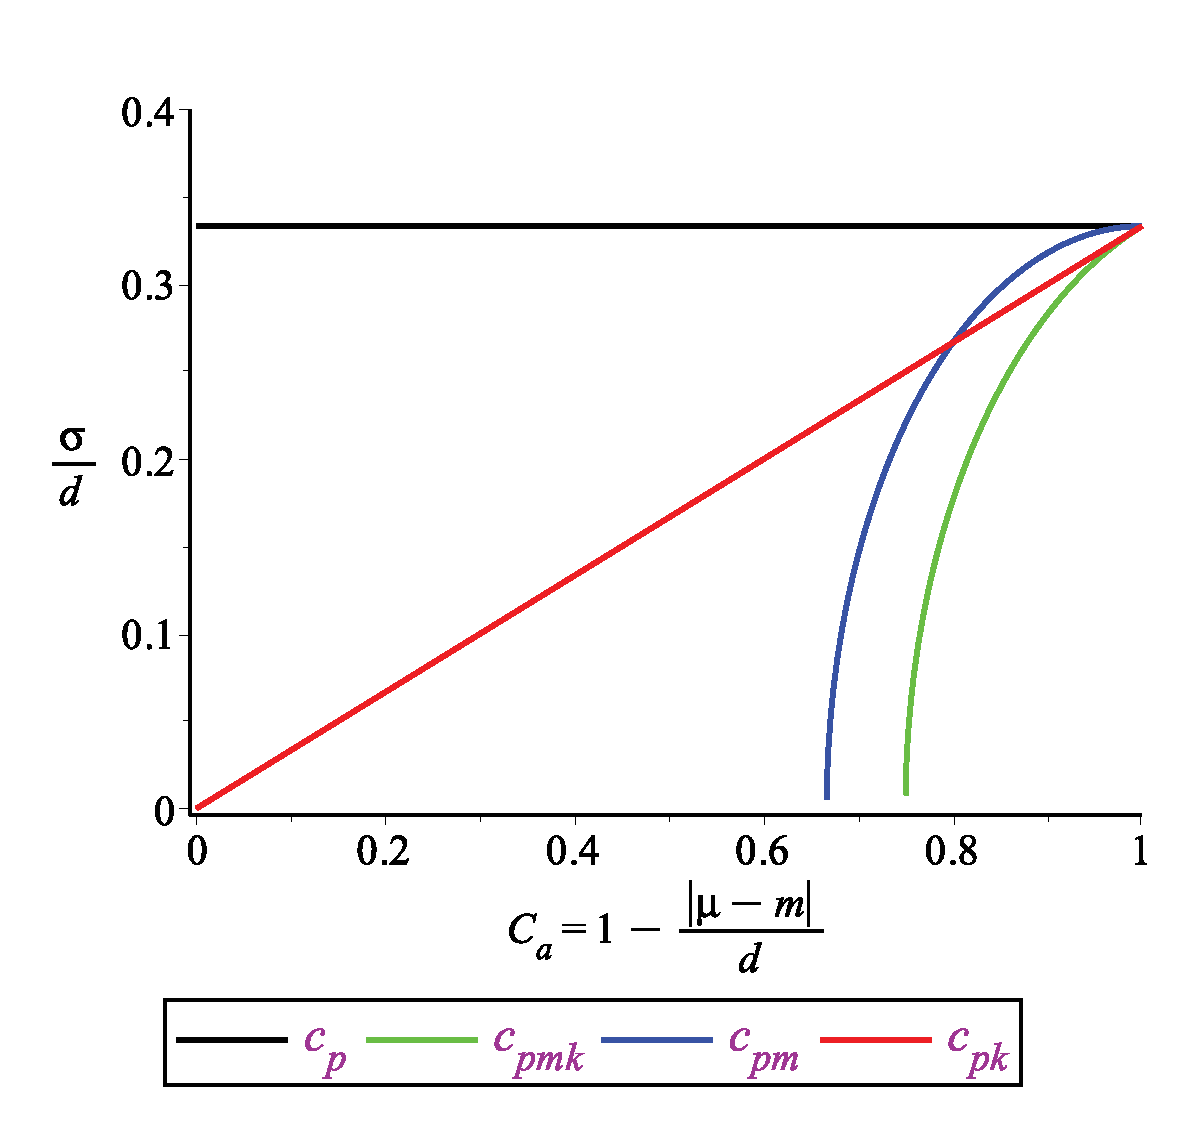
\includegraphics[width=0.5\textwidth]{graph_postscript_test.eps}
\caption{\label{fig:cpk} $c_p$ referens only to the variance of the process. $c_{pk}$ is related to the yield of the product. $c_{pm}$ takes a loss function in to account relates to a target dimension. $cpmk$ takes both the yield of the product and a loss function. }
\end{figure}

sample size  \ref{eq:sddj}




Obtaining Process Capability data is a process of measuring a lot of products.
Products are measured and compared to the nominal size they were produced for, this is called error.

In a production line control measurement are usually done by taking a set of samples to represent the entire population. Each product in the sample set, produces a measurement. From the set of measurements a standard deviation and a mean shift is calculated.

\section{uses}
existance of it-grade
improvement per rework
material selection





By looking at normalized data of the variance of products of the same material and process, it is possible to find a suitable tolerance

\section{implementation}





A cross company platform is suggested to populate the database. The gain is diverse data to be able to compare materials and processes. 

Even relatively big companies in Denmark does not have the resources record 

Since companies tends to be conservative in their production 
By 

The more data the better. The GPC tool's strength is the ability of draw knowledge from actual components of big diversity. Allowing  

In a production company structure consisting of a Production unit, a Mechanical Design unit and a Quality Reassurance unit, the Quality 

A change in the existing system has to be made is .
 

\cite{perzyk1998selection}

To populate GPC 

Industry secretsxcxc
	experience
	
	
active actors and interest groups
	sub suppliers 
	mechanical design consultants
	

difficulties
	Non disclusure agreement
	end-customer
	

\section*{References}
\bibliography{../PCDBmasterBibliography/PCDB_Master_bib.bib}

\end{document}